
% This LaTeX was auto-generated from an M-file by MATLAB.
% To make changes, update the M-file and republish this document.

%%% \documentclass{article}
%%% \usepackage{graphicx}
%%% \usepackage{color}

%%% \sloppy
%%% \definecolor{lightgray}{gray}{0.5}
\setlength{\parindent}{0pt}

%%% \begin{document}

    
    
\subsection*{Windowed Discrete Fourier Transform}

\begin{par}
Example for algorithm SP-WFFT.
\end{par} \vspace{1em}
\begin{par}
Windowed Discrete Fourier Transform is method to calculate frequency and phase spectrum. Example shows the effect of coherent sampling, non-coherent sampling, windowing and zero padding on estimating amplitude and phase by means of FFT. Last part compares all windows in frequency space.
\end{par} \vspace{1em}

\subsubsection*{Contents}

\begin{itemize}
\setlength{\itemsep}{-1ex}
   \item Generate sample data
   \item Call algorithm
   \item Display results
   \item Compare window coefficients
\end{itemize}


\subsubsection*{Generate sample data}

\begin{par}
Construct 1 second of signal sampled at 50 Hz containing two harmonic components at 1 and 8 Hz and one interharmonic component at 15.5 Hz with various amplitudes and phases.
\end{par} \vspace{1em}
\begin{lstlisting}[style=mcode]
clear DI
DI.fs.v = 50;
fnom = [1;   8; 15.5];
Anom = [1; 0.5;  0.3];
pnom = [0;   1;    2];
DI.t.v = [0 : 1/DI.fs.v : 1 - 1/DI.fs.v];
DI.y.v = zeros(size(DI.t.v));
for i = 1:length(fnom)
        DI.y.v = DI.y.v + Anom(i).*sin(2.*pi.*fnom(i).*DI.t.v + pnom(i));
end
%
\end{lstlisting}


\subsubsection*{Call algorithm}

\begin{par}
Calculate amplitude and phase spectrum and store results into \lstinline{DO}. Window function is not specified, therefore rectangle (none) window will be used.
\end{par} \vspace{1em}
\begin{lstlisting}[style=mcode]
DO = qwtb('SP-WFFT', DI);
%
% Set window function to blackman and calculate windowed amplitude and phase spectrum and store results into |DOw|.
DI.window.v = 'blackman';
DOw = qwtb('SP-WFFT', DI);
%
% Set zero padding to 10 times the signal length and calculate zero padded windowed amplitude and
% phase spectrum and stre results into |DOwz|.
DI.fft_padding.v = 10.*length(DI.y.v);
DOwz = qwtb('SP-WFFT', DI);
%
\end{lstlisting}

        \begin{lstlisting}[style=output]
QWTB: no uncertainty calculation
QWTB: no uncertainty calculation
QWTB: no uncertainty calculation
\end{lstlisting} \color{black}
    

\subsubsection*{Display results}

\begin{par}
Plot amplitude spectrum.
\end{par} \vspace{1em}
\begin{lstlisting}[style=mcode]
figure; hold on;
plot(fnom, Anom, '+r', 'markersize', 10, 'linewidth', 2);
stem(DO.f.v, DO.A.v, '-ob', 'filled', 'markersize', 3);
plot(DOw.f.v, DOw.A.v, '-g','linewidth',2);
plot(DOwz.f.v, DOwz.A.v, '-k');
legend('nominal values','FFT', 'blackman window', 'blck. w. + zero padding')
title('Amplitude spectrum')
xlabel('frequency (Hz)'); ylabel('amplitude (V)');
hold off
% Plot phase spectrum
figure; hold on;
plot(fnom, pnom, '+r', 'markersize', 10, 'linewidth', 2);
stem(DO.f.v, DO.ph.v, '-ob', 'filled', 'markersize', 3);
plot(DOw.f.v, DOw.ph.v, '-g','linewidth',2);
plot(DOwz.f.v, DOwz.ph.v, '-k');
legend('nominal values','FFT', 'blackman window', 'blck. w. + zero padding', 'location', 'southwest')
title('Phase spectrum');
xlabel('frequency (Hz)'); ylabel('phase (rad)');
hold off
%
\end{lstlisting}

\begin{center}
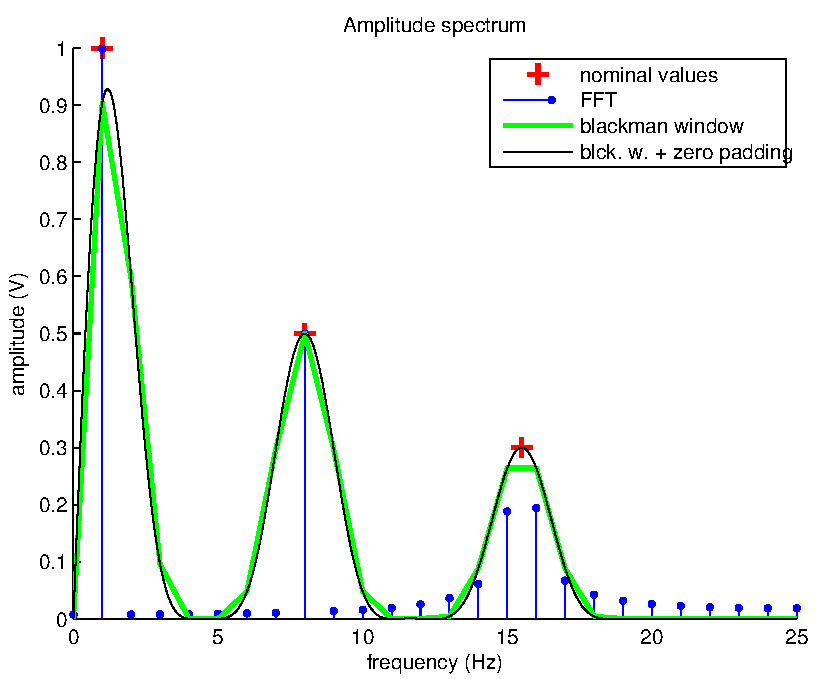
\includegraphics[width=0.7\textwidth]{algs_examples_published/SP-WFFT_alg_example_01.pdf}
\end{center}

\begin{center}
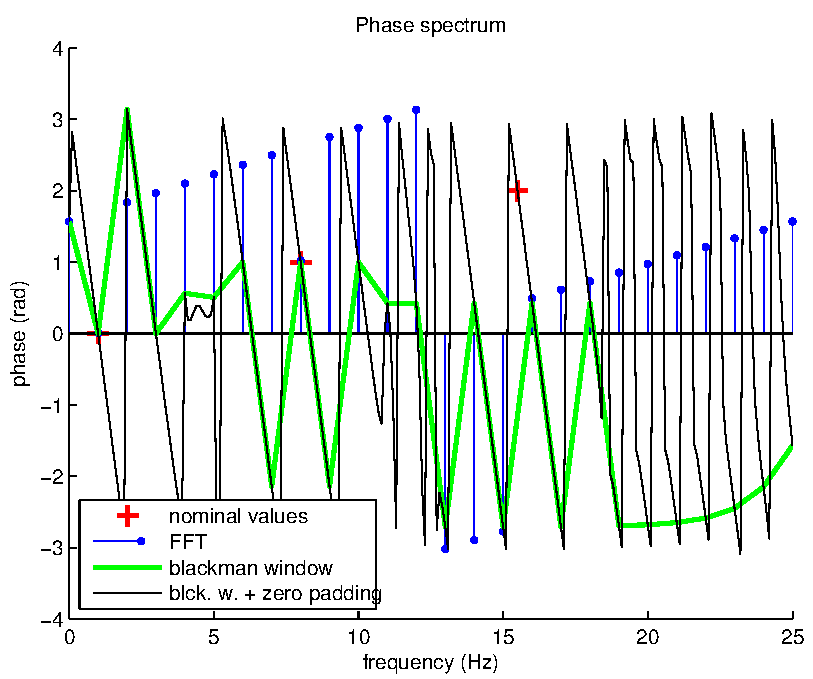
\includegraphics[width=0.7\textwidth]{algs_examples_published/SP-WFFT_alg_example_02.pdf}
\end{center}


\subsubsection*{Compare window coefficients}

\begin{par}
Different windows has different peak widths, heights of side lobes and side lobes roll off ratio. To see the window differences a zero padding is used. First a simple signal of ones is prepared and zero padding is specified to 100x the length of signal. Next for every window a spectrum is calculated and plotted.
\end{par} \vspace{1em}
\begin{lstlisting}[style=mcode]
clear DI
DI.y.v = ones(1,10);
DI.fs.v = 1;
DI.fft_padding.v = 100.*length(DI.y.v);
avail_windows = {'barthann' 'bartlett' 'blackman' 'blackmanharris' 'blackmannuttall' 'bohman' 'cheb' 'flattop_matlab' 'flattop_SFT3F' 'flattop_SFT4F' 'flattop_SFT5F' 'flattop_SFT3M' 'flattop_SFT4M' 'flattop_SFT5M' 'flattop_248D' 'gaussian' 'hamming' 'hanning' 'kaiser' 'nuttall' 'parzen' 'rect' 'triang' 'tukey' 'welch'};
col = jet(length(avail_windows));
figure; hold on;
for i = 1:length(avail_windows)
        DI.window.v = avail_windows{i};
        DO = qwtb('SP-WFFT', DI);
        plot(DO.A.v, '-', 'color', col(i,:));
end
h=legend(avail_windows);
h=legend('location','eastoutside');
set(h,'FontSize',8, 'interpreter','none');
xlabel('FFT bin * 100');
ylabel('amplitude');
hold off;
\end{lstlisting}

        \begin{lstlisting}[style=output]
QWTB: no uncertainty calculation
QWTB: no uncertainty calculation
QWTB: no uncertainty calculation
QWTB: no uncertainty calculation
QWTB: no uncertainty calculation
QWTB: no uncertainty calculation
QWTB: no uncertainty calculation
QWTB: no uncertainty calculation
QWTB: no uncertainty calculation
QWTB: no uncertainty calculation
QWTB: no uncertainty calculation
QWTB: no uncertainty calculation
QWTB: no uncertainty calculation
QWTB: no uncertainty calculation
QWTB: no uncertainty calculation
QWTB: no uncertainty calculation
QWTB: no uncertainty calculation
QWTB: no uncertainty calculation
QWTB: no uncertainty calculation
QWTB: no uncertainty calculation
QWTB: no uncertainty calculation
QWTB: no uncertainty calculation
QWTB: no uncertainty calculation
QWTB: no uncertainty calculation
QWTB: no uncertainty calculation
\end{lstlisting} \color{black}
    
\begin{center}
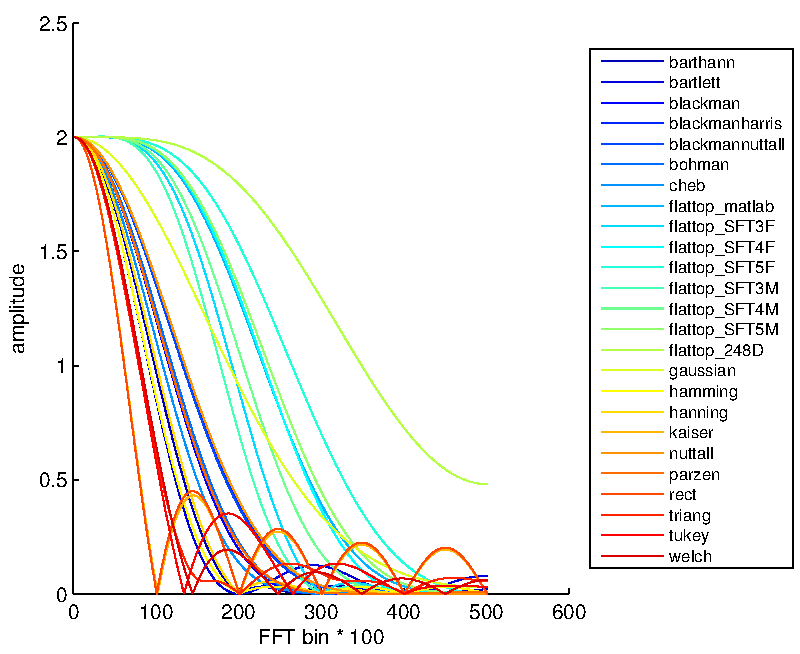
\includegraphics[width=0.7\textwidth]{algs_examples_published/SP-WFFT_alg_example_03.pdf}
\end{center}



%%% \end{document}
    
